\subsection{Geometría de la Constelación y Dinámica de Rotación en FSK}
La Figura 11 corrobora que la FSK posee una envolvente constante, trazando una circunferencia en el plano I/Q cuya geometría es invariante ante la portadora ($f_c$), validando la independencia analítica de la Envolvente Compleja. Adicionalmente, la desviación de frecuencia ($f_d$) rige la velocidad angular del vector: para $f_d = 2$ kHz (Fig. 11a), el leve desplazamiento de fase entre muestras concentra los puntos en un arco denso; al incrementar a $32$ kHz (Fig. 11b), la rápida rotación dispersa las muestras sobre toda la trayectoria. Esto evidencia que la información subyace puramente en la tasa de cambio de la fase instantánea.
\begin{figure}[H]
    \centering
    \subfloat[Desviación de 2 kHz: Alta densidad de puntos en un arco reducido.]{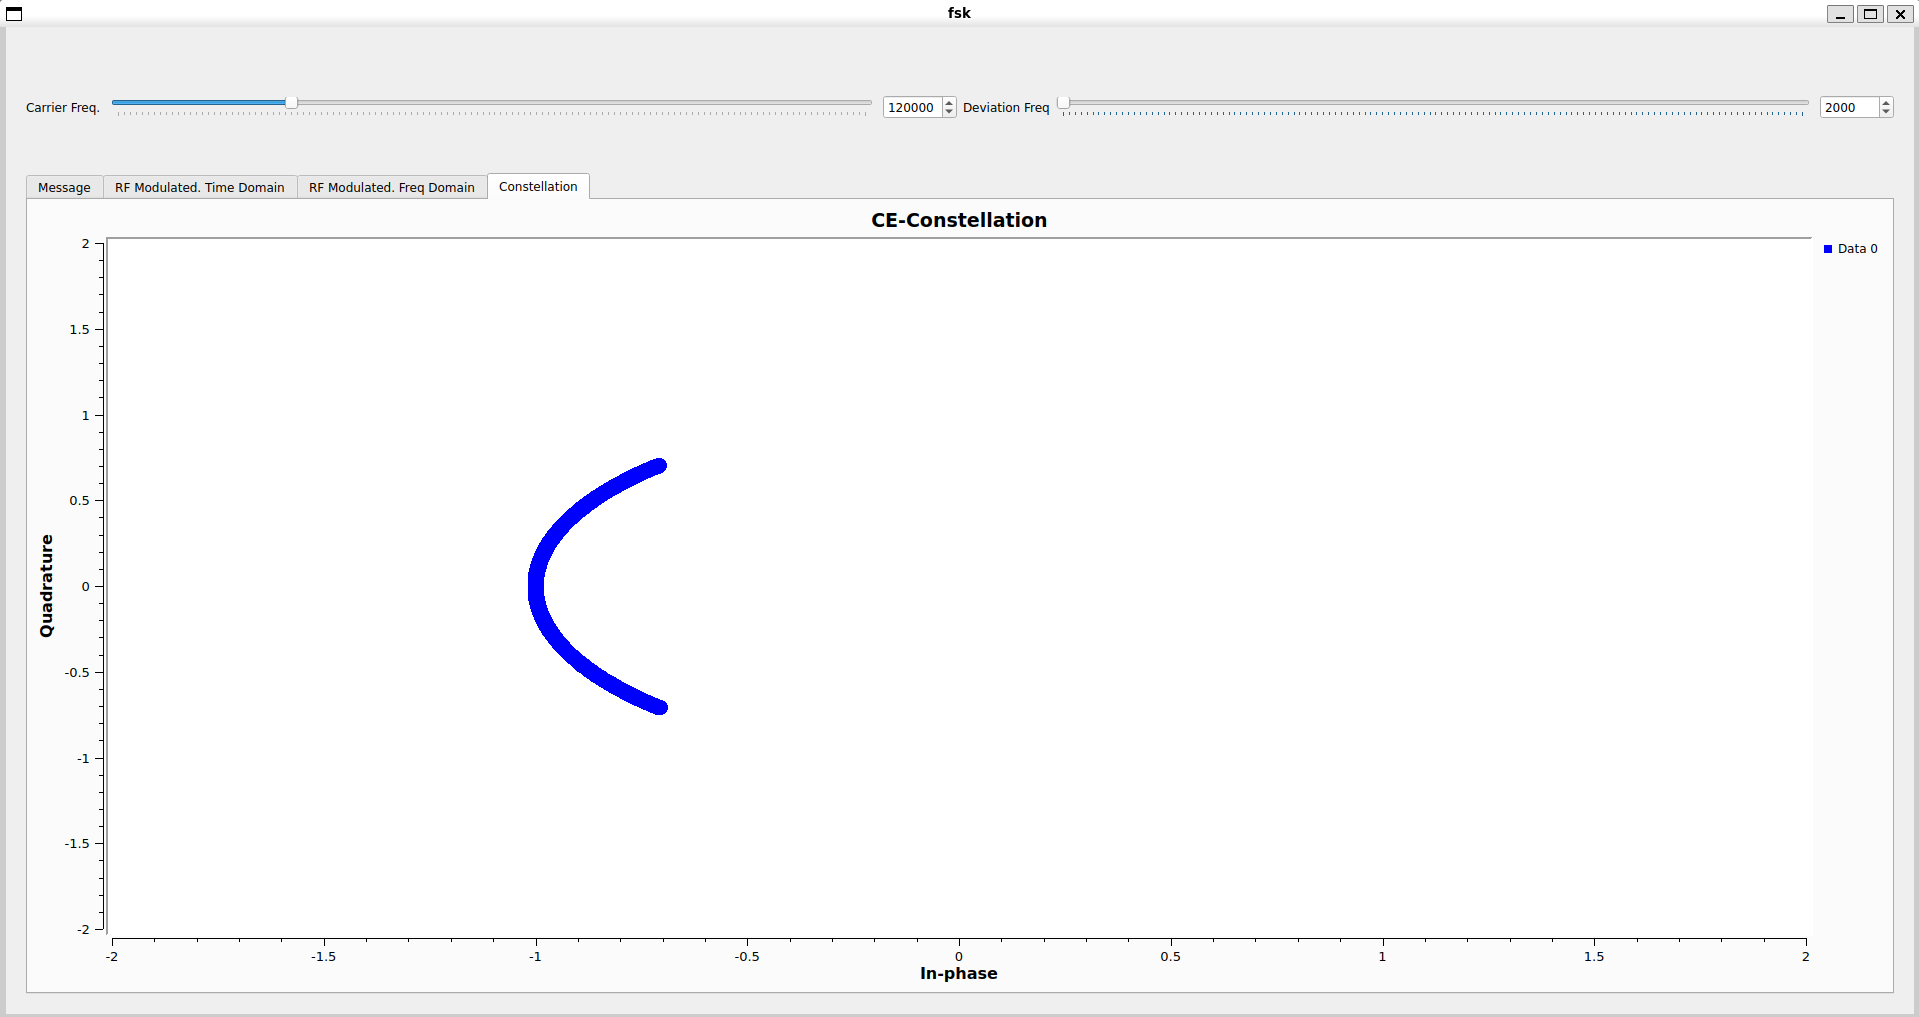
\includegraphics[width=0.48\linewidth]{imagenes/constelacion_punto_8_fc_12000_df_2000.png}\label{fig:const_2k}}
    \hfill
    \subfloat[Desviación de 32 kHz: Puntos esparcidos por la rotación acelerada.]{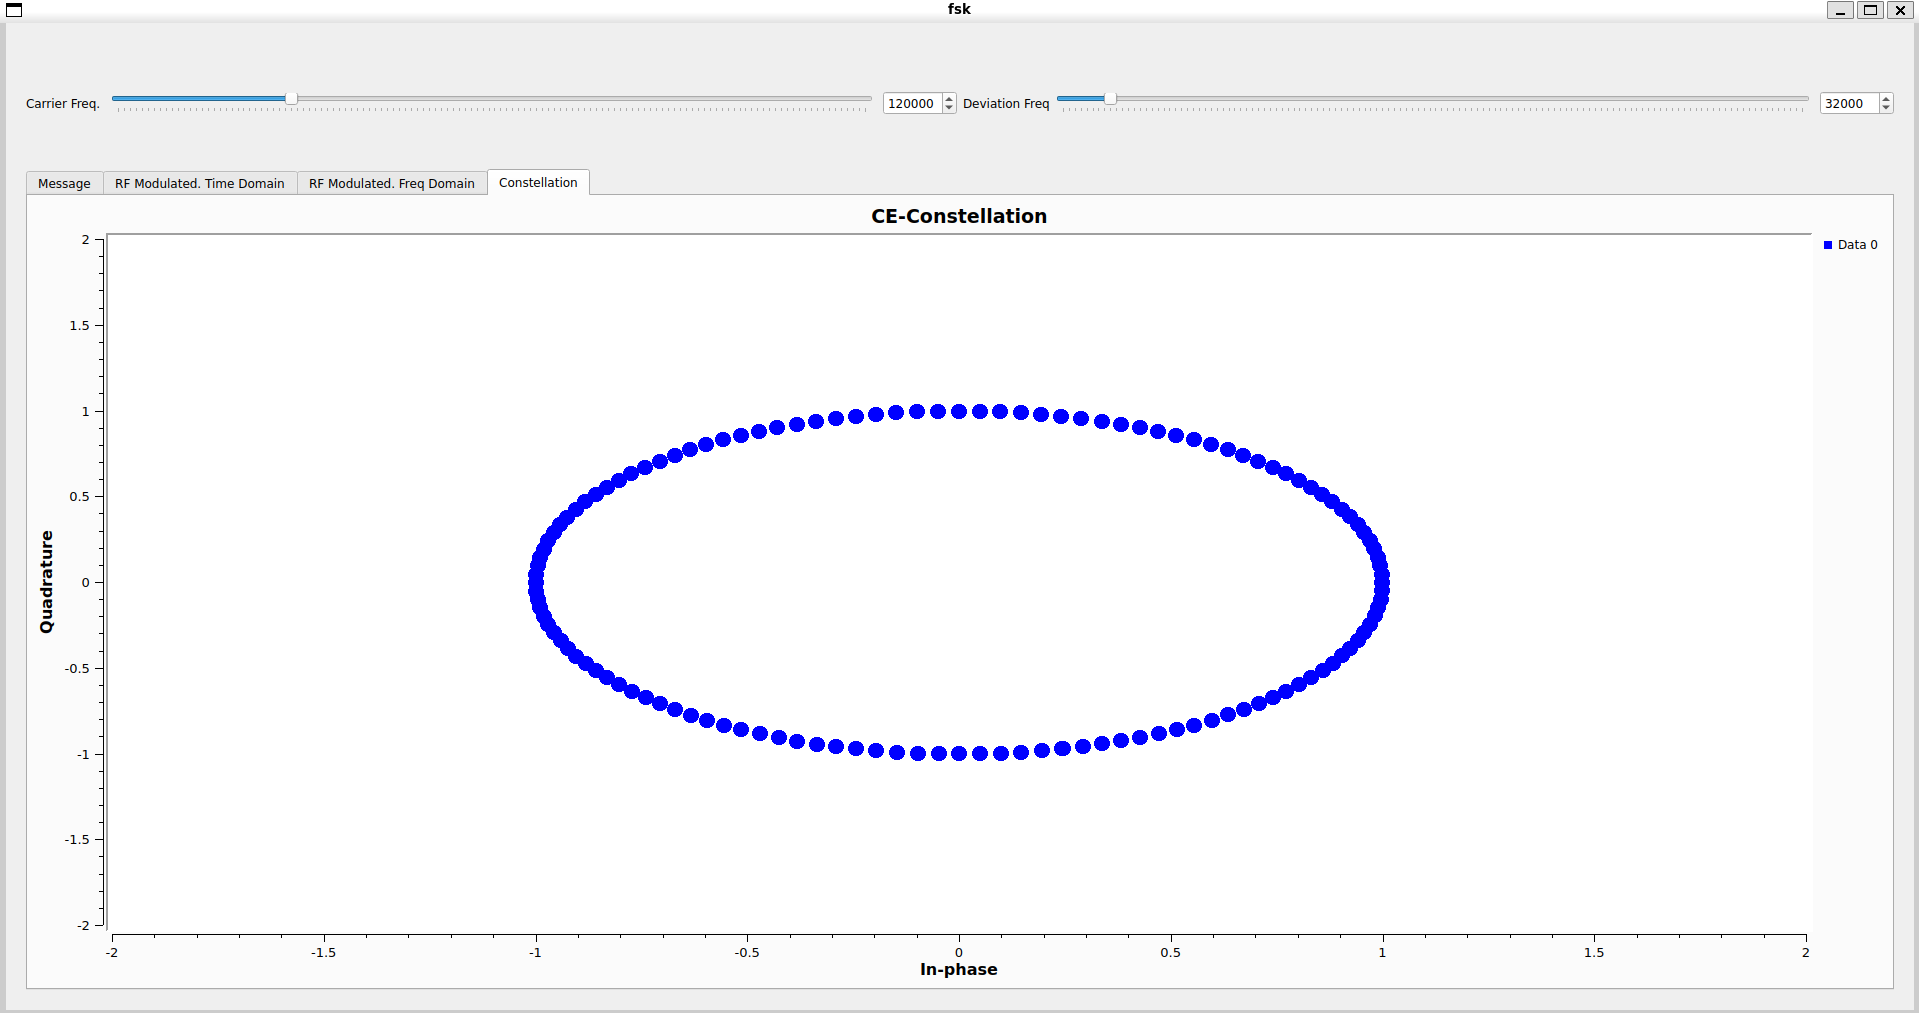
\includegraphics[width=0.48\linewidth]{imagenes/constelacion_punto_8_fc_12000_df_32000.png}\label{fig:const_32k}}
    \caption{Trayectorias de fase en el plano complejo para diferentes niveles de desviación.}
    \label{fig:constelaciones}
\end{figure}